\chapter{Haptic texture rendering}
\label{haptic}
\thispagestyle{empty}% no page number in chapter title page

The human haptic perception system relies on kinesthetic and cutaneous sensory information provided by several receptors during probe-surface interactions \cite{leder09}.
 
The kinesthetic sense focuses on the perception of forces and torques acting on the human
body. Kinesthetic stimulation is sensed by mechanoreceptors located in the muscles. Kinesthetic mechanoreceptors include muscle spindles in parallel with muscle fibers and Golgi tendon organs in series with them at the connection with the skeleton \cite{rahul15}. In some mainly kinesthetic tasks, the tactile sense only indicates a contact.

Tactile perception is stimulated by cutaneous receptors. There are four kinds of mechanoreceptors in the glabrous skin: The Merkel cells (Braille dots and sharp edges), Meissner corpuscles (low-frequency vibrations), Pacinian corpuscles (high frequency stimuli), Ruffini endings (still unknown).

Friction, hardness, macroscopic roughness, microscopic roughness and thermal conductivity are the main dimensions to build haptic texture models. All of these aspects should be well considered in order to increase immersion into a virtual environment. In the following of this thesis, microscopic roughness is our main focus as a vibrotactile feature.

\section{Roughness}

As an abstract feature roughness plays an important role in haptic signal perception.The roughness dimension may be divided into two dimensions: macro and fine (micro) roughness as in \cite{okamoto13}.

\subsection{Macroscopic Roughness}

Due to the duplex nature of roughness,  macroscopic roughness should strictly be considered in order to understand fine roughness. Coarse roughness is mainly represented by the ``uneven'', ``relief'', or ``voluminous'' labels and mediated by different mechanisms from micro roughness. For coarse surface roughness, the spatial  distribution of SAI units is related to roughness perception \cite{okamoto13}.

\subsection{Fine Roughness}

In the mechanism of fine roughness perception, FAI and FAII units contribute and is mainly represented by the ``rough" label. During surface-tool or surface-finger sliding motions, high frequency vibrations can be extracted using an accelerometer mounted on a human finger. Microscopic roughness impressions can be characterized by these vibrations. The macro and fine roughness dimensions can be separated according to the mentioned aspects but can intersect each other during the process of perception.  Figure \ref{fig:texture} illustrates the process of texture production with an accelerometer.
\begin{figure}[h!]
	\begin{center}
		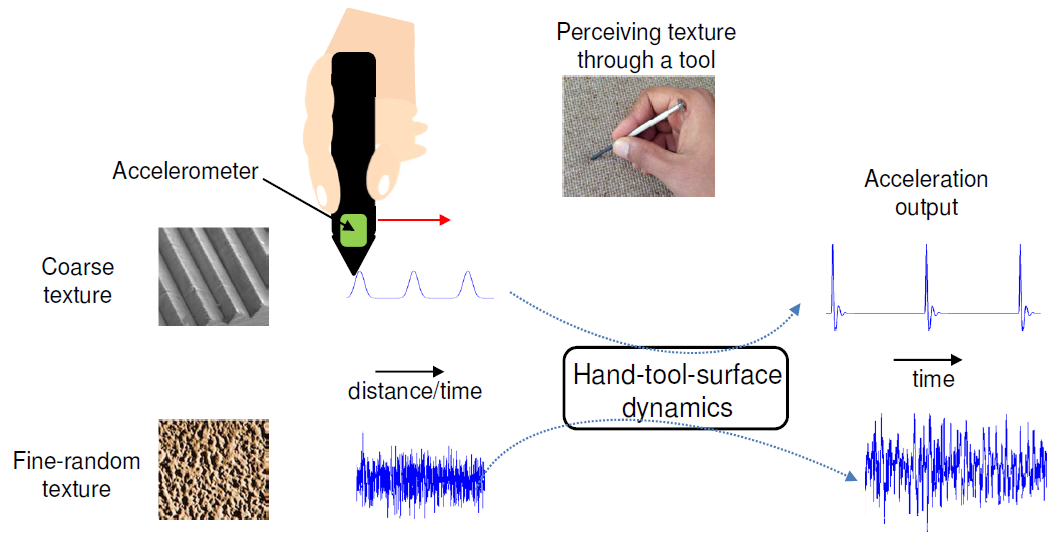
\includegraphics[width=14cm]{texture}
		\caption{Mechanism of texture production. A hand-held tool is used to stroke a textured surface. An acceleration sensor signal mounted on the tool measures the response of the hand-tool system as it hits surface features. Figure reproduced from \cite{rahul15} }
		\label{fig:texture}
	\end{center}
\end{figure}

The recorded acceleration signals depend on the scan speed and force, nonetheless we ignore the force dependencies as mentioned in the introduction part. Thereby, our approach in this thesis is generating vibrotactile signals based on the recorded acceleration data for different absolute scan speed. They are then displayed via a voice coil actuator. 


\chapter{Interpolation of vibrotactile signals}
\label{interpolation}

Priori model designs have recently been evolved into data-driven haptic textures. The apparent concept is simply displaying recorded texture acceleration signals, where the exploratory speed dependency is disregarded. However, this is not a sufficient way of representing acceleration response. Therefore, user speed should be incorporated into the feedback signal.

As in \cite{refined12} is described, there are some methods of relating speed variable to tactile signals such as switching between recordings according to speed, which may however be perceptually detectable. Another way is building a function depending on speed that gives a weighted average of recorded acceleration signals as output. The problem that may occur here is that the frequency content is not preserved due to the probable constructive and destructive interference between signals. These aspects create the idea of data-driven texture models.

In the following, we analyze two methods for synthesizing vibrotactile signals without creating noticeable artifacts. The first method is synthesizing two recorded acceleration signals under different speed conditions through LPC method and interpolating between them by linear interpolation of filter variables. The second one is reproducing these two signals from their major frequencies and interpolating between them according to the major frequencies.

In the following, we go deep into both of the principles and how to apply them to produce interpolated signals.

\section{Linear predictive coding}
The basic idea of Linear Predictive Coding (LPC) is to develop a transfer function that can predict each sample of a signal as a linear combination of the previous samples. It has applications in filter design and speech coding. 

We consider an IIR filter $H(z)$ of length n in the form $H(z)=[-h_1z^{-2}-h_2z^{-1}...-h_nz^{-n}]$.
Our acceleration data vector from PCA is called {$\vec{a}(k)$} in the following. The resulting prediction vector from our filter is $\vec{\hat{a}}(k)$. The residual signal {$\vec{e}(k)$} is the difference between these two signals.The transfer function $P(z)$ is the result of the following equation:

\begin{equation} \label{eq:transferfunction}
\frac{\vec{e}(k)}{\vec{a}(k)}=1-H(z)=P(z)   
\end{equation}

It is possible to compute the residual at each step using the vector of filter coefficients $\vec{h}=[h_1 h_2 h_3 ... h_n]^T$:

\begin{equation} \label{eq:residual}
\vec{e}(k)=a(k)-\hat{a}(k)=a(k)-\vec{h}^T\vec{a}(k-1)   
\end{equation}

At this step, we aim to find the minimum value of the residual function $e(k)$. We are able to reduce the problem to Wiener-Hopf equation by a cost function based on mean-square error. The Wiener-Hopf equation can be solved by Levinson-Durbin \cite{durbin} algorithm, so that we can obtain our optimal filter vector $\vec{h_0}$. 

To synthesize new signals, we use a white noise signal {$\vec{e_g}(l)$} as input, which is filtered with $1/P(z)$, in order to generate our desired response {$\vec{a_g}(l)$}. For a better overview, we can rewrite the equations (\ref{eq:transferfunction}) and (\ref{eq:residual}) as follows:

\begin{equation}
\frac{\vec{a_g}(l)}{\vec{e_g}(l)}=\frac{1}{1-H(z)} =\frac{1}{P(z)} 
\end{equation}

\begin{equation}
a_g(l)=e_g(l)+\vec{h}^T\vec{a_g}(l-1) 
\end{equation}

Figure \ref{fig:lpc-blockdiagram} illustrates each of analyzing and synthesizing processes via block diagram. The value {$\vec{e_g}(l)$} is a randomly generated Gaussian white noise but its average signal power must be equal to that of the average signal power remaining in the residual, $P\{\vec{e}(k)\}$ after filter optimization.

\begin{figure} 
	
	\subfigure[Block diagram for prediction of the next contact acceleration $a(k)$
	given the recorded series $a(k)$ with residual $e(k)$.]{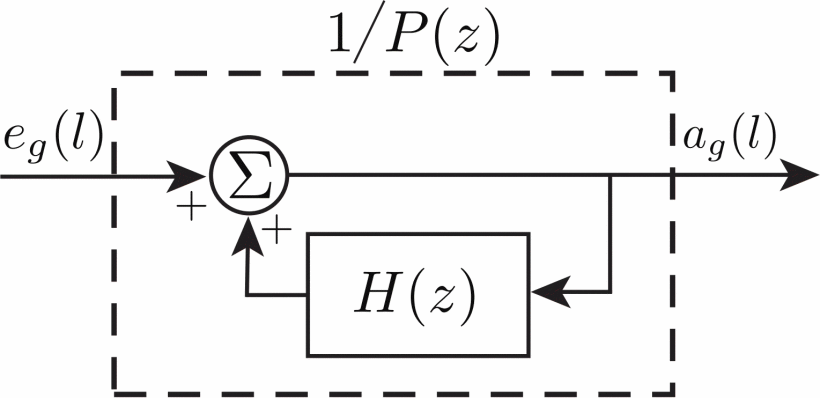
\includegraphics[width=0.49\textwidth]{lpcsynthesis}} 
	\subfigure[Block diagram for the synthesis of an acceleration signal $a_g(l)$
	from the appropriately scaled white noise input $e_g(l)$.]{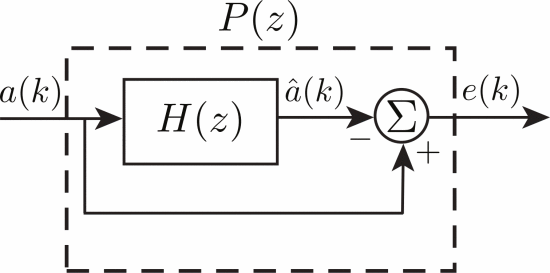
\includegraphics[width=0.49\textwidth]{lpc}} 
	\caption{Signal generation through LPC principle. Figures reproduced from \cite{romano10}.} 
	\label{fig:lpc-blockdiagram}
\end{figure} 

The definition of power is as in the following equation:

\begin{equation}
P\{\vec{a}(l)\}=\frac{1}{N}\sum_{n=0}^{N-1}|a(n)|^2
\end{equation}

This is equivalent to signal variance $\sigma�$ ,because our signals are zero-mean signals. Now, we have to determine the order of our prediction filter, which affect the accuracy of the prediction. The higher we choose the order, the smaller the residual gets. It means we have a better prediction with higher orders, but then the calculation gets  more complicated. It is possible to calculate the success of the synthetic result with a cost function defined as the RMS error as follows:

\begin{equation} \label{costfunction}
C\{\vec{a_g}(l)\}=\frac{RMS(DFT_s\{\vec{a}(l)\}-DFT_s\{\vec{\hat{{a_g}}}(l)\})}{RMS(DFT_s\{\vec{a}(l)\}}
\end{equation}

Using this equation, where $DFT_s\{\vec{a}\}$ represents the discrete Fourier transform of vector $\vec{a}$, it is possible to obtain the optimal order of the filter. In our case we choose 400 as the order for the best quality of results as in \cite{romano10}.

Now that we have generated our prediction filter with two unique variables $\vec{h}$ vector and $e_g(l)$, it comes to interpolate between our synthesized signals to create new signals. Bilinear interpolation of both the vector $\vec{h}$ and $e_g(l)$ of two signals in different velocities and applying these new values to our prediction filter result in new synthesized signals, so that we create signal data for audio signals at different force and velocities. 

\section{Signal Generation from Major Frequencies}

The other method for signal generation is using rich and valuable information of signals' high frequencies. The frequency of the vibration must change as the users change their force and so that their velocity. This is one of the realistic methods for interpolation between signals recorded under different velocities.

At first we determine the number of the frequencies we are going to deal with for synthesizing new signals. This is done in a similar way to order selection of a prediction filter in the previous section. For our case we set 20 for the optimum frequency number, which is going to be reduced as described in the following of this section.

In order to find the frequencies with highest amplitudes, we calculate the discrete Fourier transform of the two recorded data and then select twenty highest amplitudes of the transformed signals. It is important here to ensure that selected frequencies should have a certain distance to each other, because the superposition of two pure tones with slightly different frequencies can lead to beats. To avoid this phenomenon, we remove frequencies among selected ones with a difference less than ? (see Figure ?).

The remaining frequencies of the recorded signals are utilized as skeleton of new signals to be generated. We define the frequency, the angle and the amplitude of each selected sample. 

We synthesize new signals by linear interpolation of amplitudes according to the following equation:

\begin{equation} \label{synthesize}
z=z+maxA(k)*(cos(2*\pi*t*maxF(k)+maxP(k))+i*sin(2*\pi*t*maxF(k)+maxP(k)))
\end{equation}

where $maxA(k)$ represents the amplitude of selected frequencies and $maxF(k)$ the frequency, $maxP(k)$ represents the phase of selected frequencies. Signal z is zero initialized at the beginning and updated as long as a new value of frequency exists. 

Finally in both methods, we write audio data by $audiowrite$  function in Matlab using the estimated signals.

\chapter{ Dependence of Speed on Friction Coefficients}
\label{friction}

Surface stickiness compels the users to apply a lateral force during surface interactions. The friction coefficient is usually calculated as the ratio
of the required dragging force of a sensor to the pressure, or
normal force \cite{mouse18}. 

In the following, we use a Phantom Omni device to feel a surface with different friction conditions, to be able to create a speed scala for some friction coefficients. Our aim is demonstrating how user speed varies depending on friction coefficients. We then use these results to evaluate speed intervals to be created in the following of this thesis, in which different audio data is displayed. The results are shown in Figures ??.  

-plots
--evaluation.

\chapter{Data-Driven Methods for Tactile Signal Evaluation}
\label{data}

The perception of displayed haptic
information typically varies across different human subjects \cite{leder09}. Therefore,experiments with human participants and their feedbacks constitute a fundamental component of the development in haptics.

As mentioned in chapter \ref{interpolation}, we analyze two methods of synthesizing vibrotactile signals for rendering fine roughness feedback: LPC and utilizing major frequencies of records. This chapter describes a human-subject experiment to evaluate how perceptually close our synthesized vibrotactile signals to the recorded acceleration signals in a haptic environment.  
\section{Experiment I}

\subsection{Subjects and Setup}

To accomplish a stable evaluation, ten volunteer human subjects, 3 female and 7 male, participated in the experiment at seperate times. Their
ages ranged from 19 to 29, with an average of 23 years. The subjects were all right-handed with limited experience with haptic devices. None
of them reported having any ailments that would affect the experiment.

We used the voice coil actuator ? in the experiment to display vibrotactile signals. 5 objects were relevant for this experiment as shown in the tabular below.

\begin{center}
	
	\begin{tabular}{||c c||} 
		\hline
		Material & Friction \\ [1ex] 	
		\hline\hline
		Coarse foam & 6   \\ 
		\hline
		2 & 7  \\
		\hline
		3 & 545  \\
		\hline
		4 & 545  \\
		\hline
		5 & 88 \\  
		\hline
	\end{tabular}
\end{center}

\subsection{Procedure}

The subject sat at a table in front of the voice coil actuator. At first, the recorded signals of each 5 different materials are displayed before the syntesized ones.

 the tactile properties of the
real and the artificially displayed surface materials for individual
subjects need to be compared and evaluated.




\chapter{Tactile Signal Speed Dependency Evaluation}





---
Bahsedilen modellerden lpcnin interpolasyonu kanitlandi.majora bakicaz deneyde.
---
 

We explain how to apply the mathematical principles of Linear
Predictive Coding (LPC) to develop a discrete transfer function that represents the acceleration response
under specific probe-surface interaction conditions. We then use this predictive transfer function to generate
unique acceleration signals of arbitrary length. In order to move between transfer functions from different
probe-surface interaction conditions, we develop a method for interpolating the variables involved in the
texture synthesis process. Finally, we compare the results of this process with real recorded acceleration
signals, and we show that the two correlate strongly in the frequency domain.


These vibrations depend on the motions of the tool and respond
to both normal force and tangential speed. This paper explores
various methods of simulating haptic texture interactions by
rendering tool vibrations that are based on recorded data. We
designed and ran a human-subject study (N=15) to analyze the
importance of creating virtual texture vibrations that respond
to user force and speed. Our analysis of data from fifteen
textures showed that removing speed responsiveness did cause
a statistically significant decrease in perceived realism, but
removing force responsiveness did not. This result indicates
that virtual textures aiming to simulate real surfaces should
vary the rendered vibrations with user speed but may not need
to vary them with user force.
that represents the acceleration response under specific probe-
surface interaction conditions. 

statistically significant decrease in realism
this study elucidated the conditions necessary
to create realistic haptic textures.
 a process of synthesizing probe-surface
interactions from data recorded from real interactions.
via automated analysis of real recorded
data.
While haptic feedback is known to increase the immersion into
a virtual environment (VE), most haptic feedback devices lack
the ability to display multidimensional tactile impressions.
To provide a more efficient and robust method of building haptic texture models from tool-surface interaction data...



 

\begin{equation} \label{eq:isim}
mRG = {\beta \cdot \sum_{k=1}^K \sum_{l=1}^L \hat{\textbf{X}}(k,l)}
\end{equation}

Durch die \texttt{\bslash label} kann auf die Bilder mit
\texttt{\bslash ref} verwiesen werden.


\section{Beispiele f�r Referenzen}
Die Literaturhinweise werden im Text z.B.\ folgenderma�en verwendet:\\
``..., wie in gezeigt, ...'' oder ``... es gibt
mehrere Ans�tze \cite{arnaud99,griswold90} ...''

\section{Schrifttypen}
Als Schrifttyp wird Arial oder Roman empfohlen. Bitte beachten, da�
Gr��en und Einheiten eine eigene Schreibweise haben:
\begin{description}
\item[Kursivschrift:] physikalische Gr��en (z.B.~$U$ f�r Spannung),
  Variablen~(z.B.~$x$), sowie Funktions- und Operatorzeichen, deren
  Bedeutung frei gew�hlt werden kann (z.B.~$f(x)$)
\item[Steilschrift:] Einheiten und ihre Vors�tze (z.B.~kg, pF),
  Zahlen, Funktions- und Operatorzeichen mit feststehender Bedeutung
  (z.B.~sin, lg)
\end{description} 

\clearpage

\section{Archivierung}
F�r die Archivierung sind alle Dateien der Arbeit (auch der Vortr�ge)
dem Betreuer zur Verf�gung zu stellen.  Weiterhin soll noch ein
\BibTeX-Eintrag der Arbeit erstellt werden (die Felder in eckigen
Klammern sind dabei auszuf�llen):
\begin{verbatim}
@MastersThesis{<Nachname des Autors><Jahr>,
  type =         {<Art der Arbeit>},
  title =        ,
  school =       {Institute of Communication Networks~(LKN),
                  Munich University of Technology~(TUM)},
  author =       {<Nachname des Autors>, <Vorname des Autors>},
  annote =       {<Nachname des Betreuers>, <Vorname des Betreuers>},
  month =        {<Monat>},
  year =         {<Jahr>},
  key =          {<Mehrere Suchschl�ssel>}
}
\end{verbatim}
